\documentclass[cjk,dvipdfmx,10pt,%
hyperref={bookmarks=true,bookmarksnumbered=true,bookmarksopen=false,%
colorlinks=false,%
pdftitle={第 54 回 関西 Debian 勉強会},%
pdfauthor={倉敷・のがた・佐々木},%
%pdfinstitute={関西 Debian 勉強会},%
pdfsubject={資料},%
}]{beamer}

\title{第 54 回 関西 Debian 勉強会}
\subtitle{{\small{資料}}}
\author[佐々木 洋平]{{\large\textbf{佐々木洋平}}}
\institute[Debian JP]{{\normalsize\texttt{関西Debian勉強会}}}
\date{{\small 2011 年 12 月 25 日}}

%\usepackage{amsmath}
%\usepackage{amssymb}
\usepackage{graphicx}
\usepackage{moreverb}
\usepackage[varg]{txfonts}
\AtBeginDvi{\special{pdf:tounicode EUC-UCS2}}
\AtBeginSection[]{\begin{frame}<beamer>\frametitle{Agenda}\tableofcontents[currentsection]\end{frame}}
\usetheme{Kyoto}
\def\museincludegraphics{%
  \begingroup
  \catcode`\|=0
  \catcode`\\=12
  \catcode`\#=12
  \includegraphics[width=0.9\textwidth]}
%\renewcommand{\familydefault}{\sfdefault}
%\renewcommand{\kanjifamilydefault}{\sfdefault}
\begin{document}
\settitleslide
\begin{frame}
\titlepage
\end{frame}
\setdefaultslide

\begin{frame}[fragile]
\frametitle{Agenda}
\tableofcontents
\end{frame}

\section{最近の Debian 関係のイベント}

\takahashi[40]{最近の\\Debian関係の\\イベント報告}

\begin{frame}[fragile]
\frametitle{第 53 回関西 Debian 勉強会}

\begin{itemize}
\item 日時: 11 月 11 - 12 日
\item 於: 関西オープンソース2011@大阪南港ATC
\end{itemize}

\begin{block}{内容}
  \begin{itemize}
  \item ブース展示, 物販: LiveCD配布. SpaceFunのポストカードが大好評.
  \item セッション1:
    「なれる!Debian開発者--45分でわかる?メンテナ入門」by やまねさん
  \item セッション2:
    「GPG キーサインパーティ」by 岩松さん
  \end{itemize}
\end{block}
\end{frame}


\begin{frame}[fragile]
  \frametitle{第82回東京エリアDebian勉強会}
  \begin{itemize}
  \item 日時: 11 月 19(土)
  \item 於: OSC 2011 Tokyo/Fall
  \end{itemize}
  \begin{block}{内容}
    \begin{itemize}
    \item ブース展示, セッション
    \end{itemize}
  \end{block}
\end{frame}

\begin{frame}[fragile]
  \frametitle{第83回東京エリアDebian勉強会}
  \begin{itemize}
  \item 日時: 12 月 17(土)
  \item 於: スクエニ
  \end{itemize}
  \begin{block}{内容}
    \begin{itemize}
    \item quilt の使い方
    \item 月刊 debhelper -- dh の使い方
    \end{itemize}
  \end{block}
\end{frame}


\takahashi[50]{そんな\\こんなで}
\takahashi[120]{次}

\takahashi[50]{事前課題発表}

\begin{frame}[fragile]
\frametitle{事前課題}

\begin{block}{今回の事前課題}
  \begin{description}
  \item[事前課題1] Debian のパッケージで「バグを発見した、けど放置してい
    る」、もしくは Debian バグ追跡システムを探索してみて興味をもったバグ
    未解決パッケージがあれば挙げてください。
  \item[事前課題2] 関西Debian勉強会で今年印象に残った話と来年聞きたい話を
    教えてください。
  \item [事前課題3] 1月に予定している関西Debian勉強会温泉合宿に参加されま
    すか。
  \end{description}
\end{block}
\end{frame}

\takahashi[50]{参加者の回答\newline 兼自己紹介}

\begin{frame}[fragile]
\frametitle{ 甲斐正三 }
  \begin{enumerate}
  \item 有りません。
  \item
    \begin{itemize}
    \item 最も印象に残った話: 第47回「ハッカーに一歩近づくTips vi編 」
      \begin{itemize}
      \item 理由1: vi(vim)は普段最もよく使っていてなじみがあるから。
      \item 理由2: 今まで使っていなかったが使うと便利なコマンドをいくつか使えるようになったから。''d100G'', ``y3G''など。
      \end{itemize}
    \item 来年聞きたい話:
      \begin{itemize}
      \item 「DebianにおけるARM Cortexとのいろいろ」
      \item Debianにおける新規CPUの開発環境構築
      \end{itemize}
    \end{itemize}
  \item 参加を希望します。
  \end{enumerate}
\end{frame}

\begin{frame}[fragile]
\frametitle{ murase\_syuka }
  \begin{enumerate}
  \item Debian バグ追跡システムを探索方法が分からない。本番までに調べてみます。
  \item パッケージ作成とかの話。blender関連のパッケージ作りたい。
  \item 未定です。
  \end{enumerate}
\end{frame}

\begin{frame}[fragile]
\frametitle{ 上川純一 }
  無回答。
\end{frame}

\begin{frame}[fragile]
\frametitle{ 山下康成 }
  \begin{enumerate}
  \item なし \_o\_
  \item
    \begin{itemize}
    \item 今年印象に残った話: そりゃ、vi でしょ(笑
    \item 来年聞きたい話:
      Developer を増やすためにも、その底辺を広げる必要があるんじゃないでしょうか。
      Debian 入門編で新しい人を呼び込みませんか。
      \begin{itemize}
      \item Windows ユーザのためのDebian 入門
      \item Debian デスクトップ入門
      \item Debian インストールハンズオン
      \item Microsoft Office ユーザのための Libre Office 入門(Debian とは関係ないか...)
        \\ ...
      \end{itemize}
    \end{itemize}
  \item 残念ながら、ますます参加できなくなった感じ
  \end{enumerate}
\end{frame}

\begin{frame}[fragile]
\frametitle{ 川江 }
  \begin{enumerate}
  \item バグではないけれど、KVMのVMの「音声」をDefaultで出るようにしてほしい。
  \item 来年はKVM関連の話が聞きたい。
  \item 参加できません。多分、San Franciscoに行ってると思います。
  \end{enumerate}
\end{frame}

\begin{frame}[fragile]
\frametitle{ 門戸良介 }
  \begin{enumerate}
  \item すみません。ありません。
  \item
    今回初めての参加です。
    仕事で初めてLinuxを使い始めてはや3年になります。
    Linuxについてさらに理解を深めようと思い関西で参加できる勉強会としてDebianの勉強会に目をつけました。
    オープンソースへの造詣は浅いですが、好奇心は強いです。勉強会の雰囲気を感じ取って、出来れば継続的な参加をしていきたいと思っています。
  \item
    参加しません。
  \end{enumerate}
\end{frame}

\begin{frame}[fragile]
\frametitle{ かわだてつたろう }
  \begin{enumerate}
  \item acpi-support: 0.138-10 に更新したらレジューム時にバックライトが点かなくなった。
  \item 運営の人になりました。
    bzr-buildpackage と git-buildpackage 話の内容とその時の会。
  \item 主催する人です。
  \end{enumerate}
\end{frame}

\begin{frame}[fragile]
\frametitle{ kozo2 }
  \begin{enumerate}
  \item
    t-code(バグを発見した、けど放置している), alien(Debian バグ追跡システムを探索してみて興味をもったバグ未解決パッケージ)
  \item
    モダンな Debian パッケージ作成入門(関西Debian勉強会で今年印象に残った話), ライセンス系の話(来年聞きたい話)
  \item
    多分参加します。
  \end{enumerate}
\end{frame}

\begin{frame}[fragile]
\frametitle{ のがたじゅん }
  \begin{enumerate}
  \item live-build 3.xでsyslinuxを使ってライブDVDを作った時、ファイル名が違うのでブートできない。
    パッチを書けばいいけど、マルチアーキの事もあるのでどう提案しようか考えたまま放置してましたが、ぼんやりこんな感じかなと思いついたので、正月にパッチを書こうかと思案中。
  \item
    ごめんなさい。今年はいろんな事があってあまり印象に残ってない…。
  \item
    考え中。温泉に行くまでが遠いので参加しないにちょっと傾きつつ…
  \end{enumerate}
\end{frame}

\begin{frame}[fragile]
\frametitle{ 佐々木洋平 }
  \begin{enumerate}
  \item sid の rubygems が ruby1.8 で動きませぬ。yaml のパースが原因なんですが、どうしたら良いかなぁ、と数日放置しています。あと地味に痛いのは squeeze の elscreen が古いままで、コマンドラインからファイルを指定して Emacs を起動できません。sid のパッケージは直っているので backports すれば良いのですが、気力がなくて放置しています。…そういや\TeX Liveの2011への移行(+日本語対応)もあったな。
  \item Debian GNU/kFreeBSD の話(杉本さん)、IPv6のトンネル話(西山さん)、でしょうか。普段自分で触らないネタなので。
    来年は月間Debian Policyとか, DFSGから始めて月間FLOSSライセンスとか, 如何?
  \item いまのところ参加する気でおりまする。
  \end{enumerate}
\end{frame}

\begin{frame}[fragile]
\frametitle{ lurdan }
  \begin{enumerate}
  \item squeeze 相当から sid に upgrade すると perl の migration に失敗する件。\#639290
  \item *-buildpackage の年だったかなぁとか。来年は月刊 debian policy なんてどうでしょう
  \item するする
  \end{enumerate}
\end{frame}

\begin{frame}[fragile]
\frametitle{ よしだともひろ }
  \begin{enumerate}
  \item sip-testerというパッケージがIPv6リンクローカルアドレスに対応していないというバグ(もしかしたら仕様?)がありますが、放置中です。(動作可能なようとなるようなパッチは作りましたが)
  \item
    \begin{itemize}
    \item 今年印象に残った話: パッケージを作るのは実はそんなに難しくはないんだということ。
    \item 来年聞きたい話: 引き続いてパッケージ作成の話と、Debian開発者となるための道のりみたいな話が聞いてみたいです。
    \end{itemize}
  \item 残念ながら参加できそうにありません。
  \end{enumerate}
\end{frame}

\begin{frame}[fragile]
\frametitle{ 金子真志 }
  \begin{enumerate}
  \item これまでは、本当に「使う」だけだったのでないです。今後は、もっと踏み込んで使ってDDになれるように頑張ります!!
  \item 今回初参加ですが、個人的なリクエストとして、「Debianパッケージの作り方〜ネットには載らないDebianDeveloper小技・テクニック〜」のような話を聞いてみたいです。(エディタのプラグインのおすすめとか・・・)
  \item 温泉合宿についてですが、学校の関係で参加したいですが、参加できなさそうです。
  \end{enumerate}
  今回初めての参加で、話についていけないかもしれませんが、これをきっかけにDebianについて学べればと思っています。
  どうぞよろしくお願いします.
\end{frame}

\begin{frame}[fragile]
\frametitle{ Y.YATSUO }
  \begin{enumerate}
  \item wicd-gtk(1.7.1~b3)の翻訳がおかしい。BTS\#651804 upstreamで既に修正されてるっぽいです。
  \item パッケージング関連が充実してましたね
  \item 極力参加する方針で…
  \end{enumerate}
\end{frame}

\takahashi[50]{そんな\\こんなで}
\takahashi[120]{次}

\section{t-code のバグレポをしてみた}
\takahashi[40]{t-code のバグレポをしてみた\\by 西田さん}

\takahashi[50]{そんな\\こんなで}
\takahashi[120]{次}

\section{さきが(ry NM 塾}

\takahashi[40]{さきが(ry NM 塾\\ by 倉敷さん}

\takahashi[50]{そんな\\こんなで}

\takahashi[50]{わしが NM 塾塾長 (ry}


\takahashi[50]{そんな\\こんなで}


\takahashi[50]{NM とは何か}

\begin{frame}[fragile]
\frametitle{NM とは何か}

\begin{block}{NM とは何か}
  \begin{itemize}
  \item 最後の一線 (Debian ユーザ的に)
  \item DM と呼ばれた後の状態 (DM 応募まだァ?)
  \item DD と呼ばれる前の状態 (DM 通過まだァ?)
  \item コネのプロセス
  \end{itemize}
\end{block}
\end{frame}

\begin{frame}[fragile]
\frametitle{NM/DD と Debian JP}

\begin{block}{NM/DD と Debian JP}
  \begin{itemize}
  \item 勉強会 (←イマココ!)
  \item GPG キーサイン
  \item DD との交流 (ふれあい)
  \item スポンサー (mentors だけでは……)
  \end{itemize}
\end{block}
\end{frame}

\takahashi[50]{ 勉強会 }
\takahashi[50]{ リア充への道、それは \\ GPG 署名 }
\takahashi[50]{ DD との交流 }
\takahashi[50]{ スポンサー }

\begin{frame}[fragile]
\frametitle{ライフワークとしての DD}

\begin{block}{ライフワークとしての DD}
  \begin{itemize}
  \item 細く長くという志向
  \item 実務的なボランティア運営の場
  \item 英語な世界へのチャンネル
  \item 地味であること
  \end{itemize}
\end{block}
\end{frame}

\takahashi[50]{ 細く }
\takahashi[50]{ 長く }
\takahashi[50]{ 実務的 }
\takahashi[50]{ 英語 }
\takahashi[50]{ 地味 }

\takahashi[40]{ ふつうの \\ おっさん \\ 問題なし }

\begin{frame}[fragile]
\frametitle{経過(1)}

\begin{block}{経過(1)}
  \begin{itemize}
  \item 2011/11 (事前ネゴ)
  \item 2011/12/04 apply
  \item 2011/12/04 advocate checked by yyabuki
  \item 2011/12/10 activity poll sent
  \item 2011/12/11 pass frontdesk precheck
  \end{itemize}
\end{block}
\end{frame}

\begin{frame}[fragile]
\frametitle{経過(2)}

\begin{block}{経過(2)}
  \begin{itemize}
  \item 2011/12/13 AM assigned to gwolf
  \item 2011/12/16 AM assigned to laney
  \item 2011/12/17 ID checked
  \item 2011/12/25 (Philosophy and Procedure やりとり中)
  \end{itemize}
\end{block}
\end{frame}

\begin{frame}[fragile]
\frametitle{Philosophy and Procedure}

\begin{block}{Philosophy and Procedure}
  \begin{itemize}
  \item 社会契約と DFSGをサマリせよ
  \item Bad licenses!
    \begin{itemize}
    \item AT\&T SCA (graphviz)
    \item qmail
    \item Creative Commons by NS-CD
    \end{itemize}
  \end{itemize}
\end{block}
\end{frame}

\takahashi[50]{ to be continued... }

\takahashi[50]{そんな\\こんなで}
\takahashi[120]{次}

\section{2011年の振り返りと2012年の企画}
\takahashi[40]{2011年の振り返りと2012年の企画\\ 司会: 佐々木}

\takahashi[50]{$<$閑話休題$>$}

\takahashi[50]{今日は忘年会です...よね?}

\takahashi[50]{$</$閑話休題$>$}

\begin{frame}[fragile]
  \frametitle{今年の振り返りと来年の計画}
  \begin{itemize}
  \item 今年のネタと参加者数を見てみる
  \item 来年のネタを考える
  \end{itemize}
\end{frame}

\begin{frame}[fragile]
  \frametitle{今年度の参加者と話題(前半)}
  \begin{tabular}{|l|c|p{18em}|}
    \hline
    開催年月  & 参加者   & 内容                                                 \\
    \hline
    2011年1月 &10        & BTS, Debian GNU/kFreeBSD                             \\
    2011年2月 &15        & pbuilder, Squeezeリリースパーティ                    \\
    2011年3月 &17        & ライセンス, Debianのドキュメント関連                 \\
    2011年4月 &25        & OSC 2011 Kansai@Kobe, \newline GPGキーサインパーティ \\
    2011年5月 &20        & vi, dpkgのおさらい                                   \\
    2011年6月 &17        & IPv6, vcs-buildpackage(svn, git)                     \\
    \hline
  \end{tabular}
\end{frame}
\begin{frame}[fragile]
  \frametitle{今年度の参加者と話題(後半)}
  \begin{tabular}{|l|c|p{18em}|}
    \hline
    開催年月  & 参加人数 & 内容                                                  \\
    \hline
    2011年7月 &17        & OSC 2011 Kansai@Kyoto, \newline GPG キーサインパーティ\\
    2011年8月 &20        & Debianパッケージ作成ハンズオン                        \\
    2011年9月 &11        & vcs-buildpackage{bzr, git}                            \\
    2011年10月&11        & Emacs, vim の拡張のDebianパッケージ, 翻訳             \\
    2011年11月&23        & KOF 2011                                              \\
    2011年12月&13        & NMプロセス, BTS (今回)                                \\
    \hline
  \end{tabular}
\end{frame}

\begin{frame}[fragile]
  \frametitle{関西Debian勉強会の参加者数の推移}
  \begin{center}
    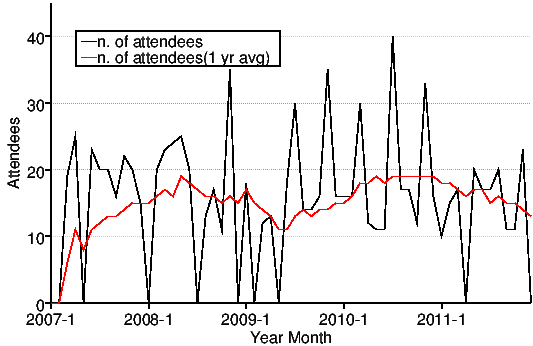
\includegraphics[width=.8\vsize]{image201112/memberanalysis/kansai.png}
  \end{center}
\end{frame}


\takahashi[50]{そんな\\こんなで}
\takahashi[120]{次}

\begin{frame}[fragile]
\frametitle{今後の予定(1)}

\begin{block}{第 55 回関西 Debian 勉強会-- Deb泉}
  \begin{itemize}
  \item 日時: 2012年 1 月 28-29
  \item 会場: 京都湯の花温泉, 温泉合宿
  \end{itemize}
\end{block}

\end{frame}

\begin{frame}[fragile]
\frametitle{今後の予定(2)}

\begin{block}{第 56 回関西 Debian 勉強会}
  \begin{itemize}
  \item 日時: 2012年 2 月 26日(日)
  \item 会場: 大阪福島区民センター
  \item 内容: 未定(募集中)
  \end{itemize}
\end{block}
\end{frame}

\takahashi[50]{  }

\end{document}
%%% Local Variables:
%%% mode: japanese-latex
%%% TeX-master: t
%%% End:
